\paragraph{Lotificación de tarimas}\label{IT-3-LotificacionDeTarimas}
\begin{steps}
    \item Verificar que el cliente esté registrado en el \gls{SGA};
    \begin{condition}
        \item[Si no está registrado:] se registra al cliente en el \gls{SGA}.
    \end{condition}

    \item El personal de embarques verifica que el lote de los registros coincidan con el lote marcado en las tarimas del producto;
    \begin{condition}
        \item[Si el lote del alimento recibido no coincide con los registros:] se le dará aviso al \emph{supervisor del almacén} para determinar que hacer.
    \end{condition}

    \item \emph{Mesa de control} registra en el \gls{SGA} los lotes del alimento y las cantidades que se almacenarán, asi como su ubicación.
    \begin{condition}
        \item[Si el alimento no tiene lote:] se le asignará un lote basado en la fecha de ingreso.
    \end{condition}

    \item \emph{\MC} genera las etiquetas para cada tarima; (\itshape ver \nameref{esp:IdTarimas}).
    \item \emph{\Emb} etiqueta las tarimas;
    \item \emph{\OP} almacena el alimento.
\end{steps}

\begin{scheme}[p]
    \centering
    \label{diag:IT-3}
    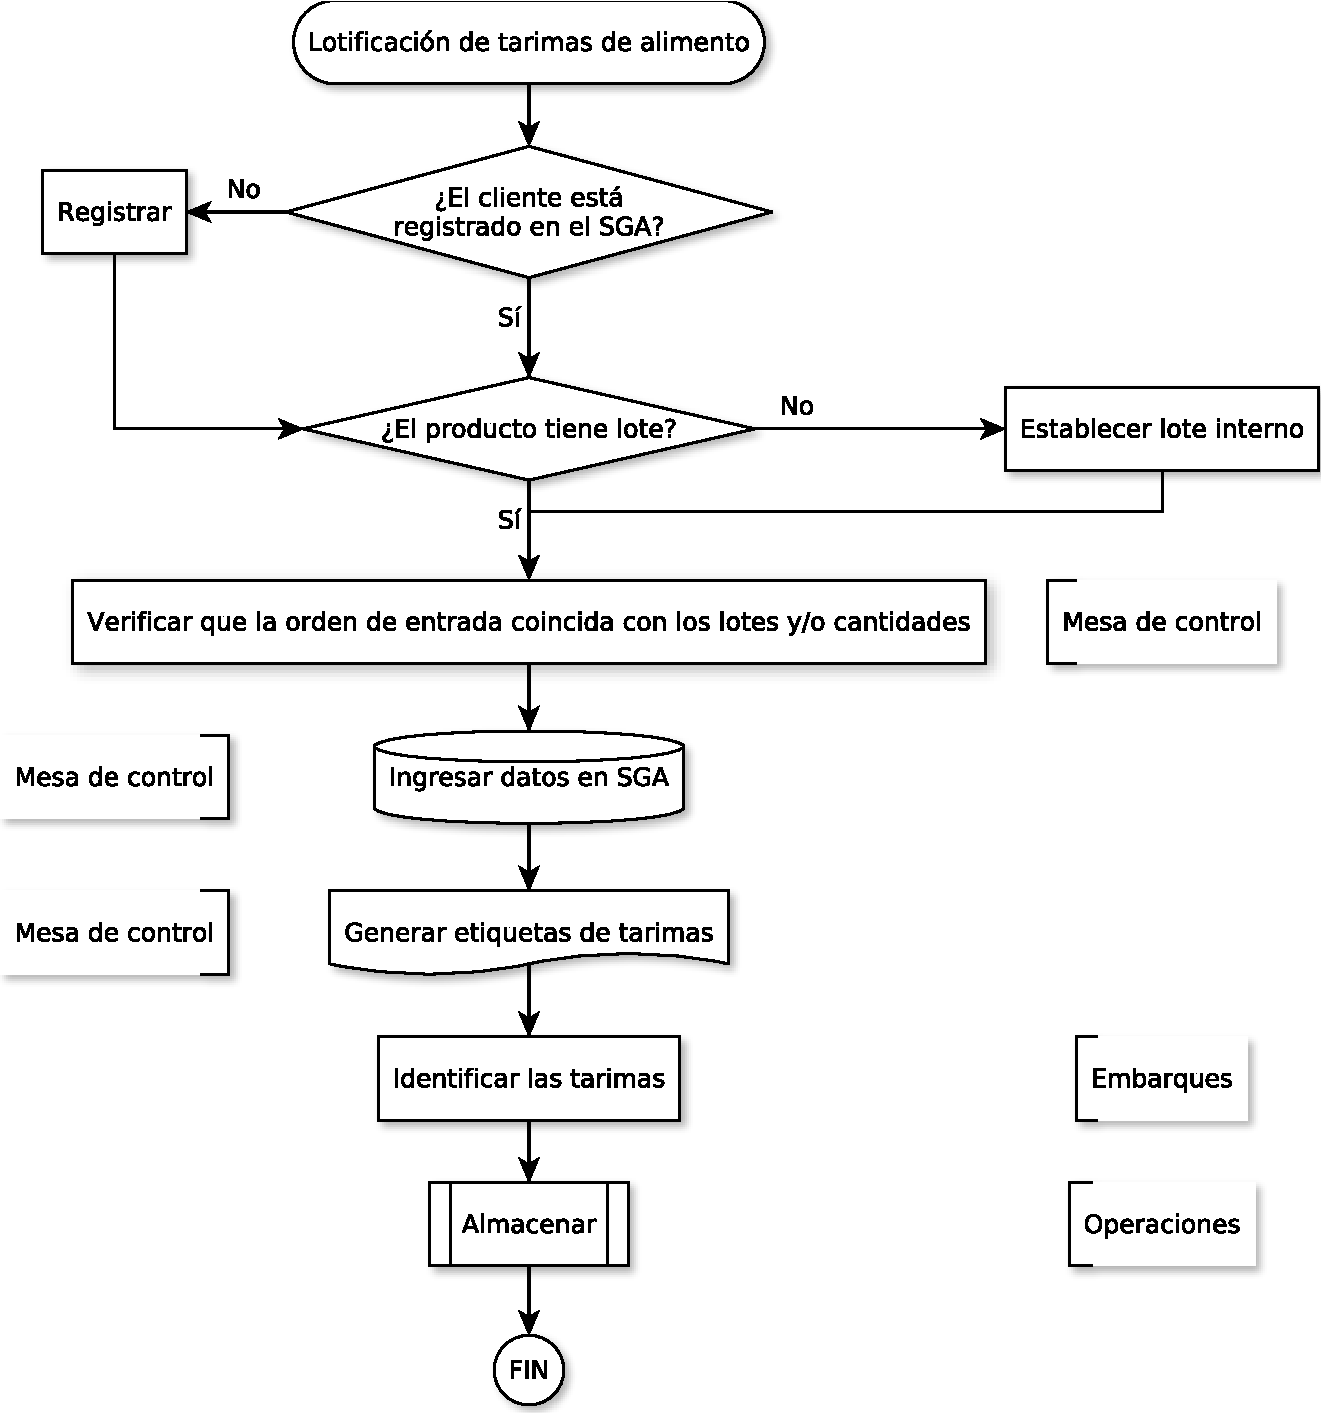
\includegraphics[width=0.9\linewidth,height=0.9\textheight,keepaspectratio]{../IT/IT-3 - Lotificación de tarimas.pdf}
    \caption[Proceso de lotificación de tarimas]{Proceso de lotificación de tarimas. Para mayor información, consultar el \cref{IT-3-LotificacionDeTarimas}.}
\end{scheme}

\begin{nota}{Identificadores de tarimas}{esp:IdTarimas}
    Las etiquetas para tarimas llevan la siguiente información:
        \begin{itemize}
            \item Fecha de recepción;
            \item nombre del cliente;
            \item nombre del alimento;
            \item fecha de caducidad;
            \item orden de compra o lote;
            \item numero de entrada;
            \item cantidad por tarima.
        \end{itemize}
\end{nota}